\let\negmedspace\undefined
\let\negthickspace\undefined
\documentclass[journal]{IEEEtran}
\usepackage[a5paper, margin=10mm, onecolumn]{geometry}
%\usepackage{lmodern} % Ensure lmodern is loaded for pdflatex
\usepackage{tfrupee} % Include tfrupee package

\setlength{\headheight}{1cm} % Set the height of the header box
\setlength{\headsep}{0mm}     % Set the distance between the header box and the top of the text

\usepackage{gvv-book}
\usepackage{gvv}
\usepackage{cite}
\usepackage{amsmath,amssymb,amsfonts,amsthm}
\usepackage{algorithmic}
\usepackage{graphicx}
\usepackage{textcomp}
\usepackage{xcolor}
\usepackage{txfonts}
\usepackage{listings}
\usepackage{enumitem}
\usepackage{mathtools}
\usepackage{gensymb}
\usepackage{comment}
\usepackage[breaklinks=true]{hyperref}
\usepackage{tkz-euclide} 
\usepackage{listings}
% \usepackage{gvv}                                        
\def\inputGnumericTable{}                                 
\usepackage[latin1]{inputenc}                                
\usepackage{color}                                            
\usepackage{array}                                            
\usepackage{longtable}                                       
\usepackage{calc}                                             
\usepackage{multirow}                                         
\usepackage{hhline}                                           
\usepackage{ifthen}                                           
\usepackage{lscape}
\usepackage{circuitikz}
\tikzstyle{block} = [rectangle, draw, fill=blue!20, 
    text width=4em, text centered, rounded corners, minimum height=3em]
\tikzstyle{sum} = [draw, fill=blue!10, circle, minimum size=1cm, node distance=1.5cm]
\tikzstyle{input} = [coordinate]
\tikzstyle{output} = [coordinate]


\begin{document}

\bibliographystyle{IEEEtran}
\vspace{3cm}

\title{9-9.7-1.3}
\author{EE24BTECH11063 - Y. Harsha Vardhan Reddy}
 \maketitle
% \newpage
% \bigskip
{\let\newpage\relax\maketitle}

\renewcommand{\thefigure}{\theenumi}
\renewcommand{\thetable}{\theenumi}
\setlength{\intextsep}{10pt} % Space between text and floats


\numberwithin{equation}{enumi}
\numberwithin{figure}{enumi}
\renewcommand{\thetable}{\theenumi}

\textbf{Question}:\\
Find the area of the region bounded by the curve $y^2=4x$ and the line $x=3$\\
\solution \\
\\
Let us first solve find the area theoretically and then verify it computationally

\textbf{Theoritical solution:}\\
Given curve,
\begin{align}
    y^2=4x
\end{align}
Area of the region bounded by $y^2=4x$ and $x=3$,
\begin{align}
   & 2 \times \int_0^3\brak{\sqrt{4x}}\cdot dx\\
   &= 2 \times 2 \times\left[ \frac{x^{3/2}}{3/2} \right]_0^3 \\
    &= \frac{8}{3} \times \sqrt{27}\\
    &= 13.856
\end{align}
The area of the region bounded between the curve $y^2=4x$ and $x=3$ is 13.856 sq.units
\textbf{Computational Solution:} Trapezoidal method\\
The difference equation for any general integral is as follows
\begin{align}    
\int_a^b f(x) \, dx \approx \frac{h}{2} \left[ f(x_0) + 2 \sum_{i=1}^{n-1} f(x_i) + f(x_n) \right]   
\end{align}
For n=1000,
\begin{align}    
\int_0^3 f(x) \, dx \approx \frac{h}{2} \left[ (2\sqrt{x_0}) + 2 \sum_{i=1}^{999} (2\sqrt{x_i}) + (2\sqrt{x_{1000})} \right]   
\end{align}
'x' varies from 0 to 3 and y varies accordingly.\\
The code sums up the required values iteratively for 'n'(say 1000) intervals\\
By computing it iteratively(computationally) we get area as 13.856 sq. units \\
Hence, the area we calculated theoretically is verified
\begin{figure}[ht!]
   \centering
   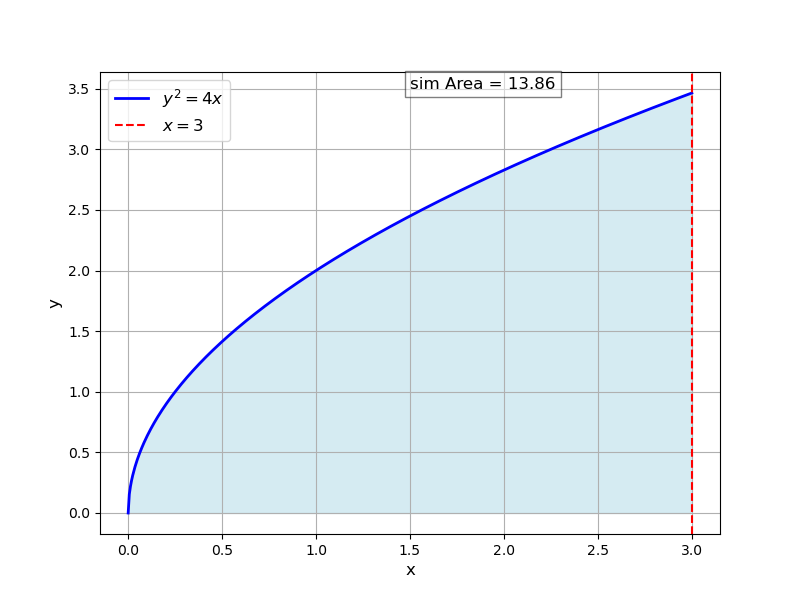
\includegraphics[width=\columnwidth]{figs/Figure_1.png}
\end{figure}
\end{document}

